\documentclass{article}
\usepackage[utf8]{inputenc}
\usepackage{amsmath}
\usepackage{amssymb}
\usepackage{amsthm}
\usepackage{enumerate}
\usepackage{mathtools}
\usepackage{float} % For plassering av bilder
\usepackage{a4wide} % mer width
\usepackage{amsmath}
\usepackage{amssymb}
\usepackage{parskip}


\usepackage[colorlinks=false,allcolors=blue]{hyperref}
%Fikser hyperref
\addto\extrasnorsk{%
\def\figureautorefname{Figure}%
\def\tableautorefname{Table}%
\def\sectionautorefname{section}%
\def\subsectionautorefname{subsection}%
}
% Vi endrer fonten som brukes for URLer til den vanlige tekstfonten.
\urlstyle{same}


% FRA IC
\usepackage{natbib}
\usepackage{amsmath}
\usepackage{listings}
\usepackage{graphicx}
\usepackage[inline]{enumitem}
\usepackage{xcolor}
 \usepackage{booktabs}
\date{}
\newcommand*{\boxednumber}[1]{%
    \expandafter\readdigit\the\numexpr#1\relax\relax
}
\newcommand*{\readdigit}[1]{%
    \ifx\relax#1\else
        \boxeddigit{#1}%
        \expandafter\readdigit
    \fi
}
% Format macro used for every digit, adjust to your liking:
\newcommand*{\boxeddigit}[1]{\fbox{#1}\hspace{-\fboxrule}}

\usepackage[left=4cm,right=4cm,vmargin=1.5cm,footnotesep=0.5cm]{geometry}
\setlength\parindent{0pt}



\title{TDT4265 - Computer Vision and Deep Learning \\Assignment 1}
\author{Jakob Vahlin & Kristian Stensgård}
%\date{September 2020}

\begin{document}

\maketitle

\tableofcontents
\newpage

\section{Theory}
\subsection{Task 1a: Derive the gradient for Logistic Regression}

\noindent We wish to derive the gradient of the \textbf{cross entropy loss} for a training set $n$, defined as

\begin{equation}
    C^n(w) = -\big(y^n \ln{(\hat{y}^n)} + (1-y^n) \ln{(1-\hat{y^n})}\big)
\end{equation}

\noindent where $\hat{y}^n = f(x^n) = \frac{1}{1+ e^{-w^T x^n}}$ is the Sigmoid activation function.


\noindent To simplify the calculations, we can split the cross entropy loss function, $C^n(w)$ into two parts,

\begin{equation}
    C^n(w) = -\big(g^n(w) + h^n(w)\big) = -\big(y^n \ln{(\hat{y}^n)} + (1-y^n) \ln{(1-\hat{y^n})}\big)
\end{equation}
\noindent by defining $g^n(w) := y^n \ln{(\hat{y}^n)}$ and $h^n(w) := (1-y^n) \ln{(1-\hat{y^n})}$. The two functions can now be differentiated separately, and their results added, due to the fact that differentiation is a linear operator. When differentiating the two functions, $g^n(w)$ and $h^n(w)$, the derivative of $f(x^n)$ w.r.t the variable $w_i$, given by \eqref{eq:known}  will be used

\begin{equation}
    \frac{\partial f\left(x^{n}\right)}{\partial w_{i}}=x_{i}^{n} f\left(x^{n}\right)\left(1-f\left(x^{n}\right)\right)
    \label{eq:known}
\end{equation}

Differentiating $g^n(w) = y^n\ln{\hat{y}^n} = y^n\ln{f(x^n)}$ gives:

\begin{align}
%\begin{split}
    \frac{\partial}{\partial w_i} g^n(w) &= \frac{\partial}{\partial w_i} y^n \ln{f(x^n)} \\
    &= y^n \Big(\frac{1}{f(x^n)} x_i^n f(x^n)(1-f(x^n))\Big) && \text{By the chain rule and \eqref{eq:known}} \\
    &= y^n x_i^n (1-f(x^n)) && \text{Cancelling terms}\label{eq:result1}
%\end{split}
\end{align}

Differentiating $h^n(w) = (1-y^n) \ln{(1-\hat{y^n})} = (1-y^n) \ln{(1-f(x^n))}$ gives:
 
\begin{align}
     \frac{\partial}{\partial w_i} h^n(w) &= 
     \frac{\partial}{\partial w_i} (1-y^n) \ln{(1-f(x^n))} \\
     &= -(1-y^n) \frac{1}{1-f(x^n)}x_{i}^{n} f\left(x^{n}\right)\left(1-f\left(x^{n}\right)\right) && \text{By the chain rule and \eqref{eq:known}} \\
     &= -(1-y^n)x_i^nf(x^n) && \text{Cancelling terms} \label{eq:result2}
\end{align}

Finally, combining the results from \eqref{eq:result1} and \eqref{eq:result2} we obtain the gradient of the cross entropy loss:

\begin{align}
    \frac{\partial}{\partial w_i} C^n(w) &= -\bigg(\frac{\partial}{\partial w_i} g^n(w) + \frac{\partial}{\partial w_i} h^n(w) \bigg) \\
    &= -x_i^n(y^n - \hat{y^n})
\end{align}

\subsection{Task 1b: Derive the gradient for Softmax Regression}

We wish to derive the gradient of the multiple class cross entropy loss function, $C^n(w)$, defined as

\begin{equation}
    C^n(w) = - \sum_{k=1}^K y_k^n \ln{\hat{y_k^n}}
    \label{eq:cn_def}
\end{equation}
where $\hat{y_k^n} = \frac{e^{z_k}^n}{\sum_{k'}^K e^{z_{k'}^n}}$, with $z_k^n = w_k^T \cdot x^n = \sum_i w_{k,i}\cdot x_i^n$. To simplify the differentiation $C^n(w)$  can be simplified in the following way

\begin{align}
    C^n(w) &= -\sum_{k=1}^K y_k^n \ln{\hat{y_k^n}} \\ 
    &= -\sum_{k=1}^K y_k^n \ln{\bigg(\frac{e^{z_k^n}}{\sum_{k'}^K e^{z_{k'}^n}}\bigg)} \\
    &= -\sum_{k=1}^K y_k^n \Bigg( \ln{(e^{z_k^n})} - \ln{\bigg(\sum_{k'}^K e^{z_{k'}^n}\bigg)} \Bigg) && \text{Logarithm quotient rule} \\
    &= -\sum_{k=1}^K y_k^n z_k^n +\sum_{k=1}^K y_k^n \ln{\bigg(\sum_{k'}^Ke^{z_{k'}^n}\bigg)} && \text{ln($e^a$) = $a$}\\
    &= -\sum_{k=1}^K y_k^n z_k^n +  \ln{\bigg(\sum_{k'}^Ke^{z_{k'}^n}\bigg)} && \text{Sum of $y^n$ entries equals 1} \label{eq:simplify_multi}
\end{align}

Similarly to Task 1a the expression in \eqref{eq:simplify_multi} can be expressed as the sum of two functions. By defining $g^n(w) := \sum_{k=1}^K y_k^n z_k^n$ and $h^n(w) := \ln{\bigg(\sum_{k'}^Ke^{z_{k'}^n}\bigg)}$  \eqref{eq:simplify_multi} can be written as

\begin{align}
    C^n(w) &= -\sum_{k=1}^K y_k^n z_k^n + \ln{\bigg(\sum_{k'}^Ke^{z_{k'}^n}\bigg)} \\
    &= -g^n(w) + h^n(w)
\end{align}

Differentiating $g(w)$ gives

\begin{align}
    \frac{\partial}{\partial w_{kj}} g(w) &= \frac{\partial}{\partial w_{kj}} \sum_{k=1}^K y_k z_k \\
    &= \frac{\partial}{\partial w_{kj}} \sum_{k=1}^K y_k \sum_{i=1}^{785} w_{ki}x_i && \text{By definition of $z_k$} \label{eq:summer}
\end{align}

By writing out a few terms of the sums in \eqref{eq:summer} we obtain

\begin{align}
\begin{split}
    \frac{\partial}{\partial w_{kj}} g(w) = \frac{\partial}{\partial w_{kj}}\Big(&y_1(w_{11}x_1 + w_{12}x_2 + \dots + w_{1i}x_i) \\
    + & y_2(w_{21}x_1 + w_{22}x_2 + \dots + w_{2i}x_i) \\
    + & y_k(w_{k1}x_1 + w_{k2}x_2 + \dots + w_{ki}x_i)  \Big)  
    \label{eq:written_out}
\end{split}
\end{align}


The derivatie w.r.t $w_{jk}$ of any given term in \eqref{eq:written_out} is only non-zero when $j=i$, in which the resutling non-zero derivative is $y_k x_j$. Thus we can conclude that

\begin{equation}
    \frac{\partial}{\partial w_{kj}} g(w) = y_k \cdot x_j\label{eq:gw}
\end{equation}

Differentiating $h(w)$ gives

\begin{align}
    \frac{\partial }{\partial w_{kj}} h(w) &= \frac{\partial }{\partial w_{kj}} \ln{\bigg(\sum_{k'}^Ke^{z_{k'}}\bigg)} \\
    &= \frac{\partial }{\partial w_{kj}} \ln{\bigg(\sum_{k'}^Ke^{\sum_{i} w_{k'i} \cdot x_i}\bigg)} && \text{By definition of $z_k'$} \\
    &= \frac{1}{\sum_{k'}^Ke^{\sum_{i} w_{k'i} \cdot x_i}} \frac{\partial }{\partial w_{kj}} \sum_{k'}^Ke^{\sum_{i} w_{k'i} \cdot x_i} && \text{By the chain rule} \label{eq:part_sum}
\end{align}

By writing out the sums of the remaining expression to be differentiated in \eqref{eq:part_sum} we obtain

\begin{align}
     \frac{\partial }{\partial w_{kj}} \sum_{k'}^Ke^{\sum_{i} w_{k'i} \cdot x_i} &=  \frac{\partial }{\partial w_{kj}} \bigg(  e^{\sum_i w_{1i}x_i} + e^{\sum_i w_{2i}x_i} + \dots + e^{\sum_i w_{Ki}x_i}\bigg) \\
     \begin{split}
     &= \Big(\frac{\partial }{\partial w_{kj}} \sum_i w_{1i}x_i \Big)e^{\sum_i w_{1i}x_i} \\ 
     &+ \Big(\frac{\partial }{\partial w_{kj}} \sum_i w_{2i}x_i \Big)e^{\sum_i w_{2i}x_i} \\
     & + \dots + \Big(\frac{\partial }{\partial w_{kj}} \sum_i w_{Ki}x_i \Big)e^{\sum_i w_{Ki}x_i} \label{eq:ledd}
     \end{split}
\end{align}

The derivative w.r.t $w_{jk}$ of any given term in \eqref{eq:ledd} is only non-zero when $j=i$ and $k = k'$, in which the resutling non-zero derivative is $x_j e^{\sum_i w_{ki}x_i}$. Thus we get

\begin{equation}
    \frac{\partial }{\partial w_{kj}} \sum_{k'}^Ke^{\sum_{i} w_{k'i} \cdot x_i} = x_j e^{\sum_i w_{ki}x_i}
    \label{eq:delres}
\end{equation}

Inserting \eqref{eq:delres} into \eqref{eq:part_sum} we obtain

\begin{align}
    \frac{\partial }{\partial w_{kj}} h(w) &= \frac{1}{\sum_{k'}^Ke^{\sum_{i} w_{k'i} \cdot x_i}} x_j e^{\sum_i w_{ki}x_i} \\
    &= \frac{e^{z_k}}{\sum_{k'}^K e^{z_{k'}}} x_j && \text{By definition of $z_k$} \\
    &= \hat{y_k}x_j && \text{By definition of $\hat{y_k}$} \label{eq:hw}
\end{align}

Finally, combining the results in \eqref{eq:gw} and \eqref{eq:hw} we obtain the gradient of the multiple class cross entrpy loss function $C^n(w)$

\begin{align}
   \frac{\partial }{\partial w_{kj}} C^n(w) &=-\frac{\partial }{\partial w_{kj}} g^n(w) + \frac{\partial }{\partial w_{kj}} h^n(w)  \\
   &= -y_k^n x_j^n + \hat{y_k^n}x_j^n \\
   &= -x_j^n(y_k^n - \hat{y_k^n})
\end{align}

\newpage

\section{Logistic Regression through Gradient Descent}
\subsection{Task 2b: Training loss}
Logistic regression with mini-batch gradient descent for a single layer neural network has been implemented. During training the training loss for each gradient step has been tracked. Additionally the validation loss over the whole validation set has been tracked for every time the network has progressed through 20\% of the training set. The loss results are shown in \autoref{fig:2bloss}. The results show that the model converges quite fast, and the validation set showing a more consistent performance. However both sets have clearly unwanted high spikes. With the training set having a higher frequency of spikes. More details on these spikes will follow in task 2e.

\begin{figure}[H]
    \centering
    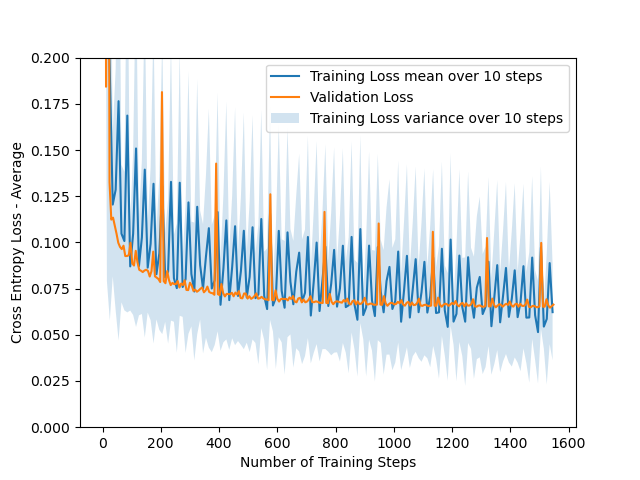
\includegraphics[width = \textwidth]{Assignment_1/Assignments/plots/task2abc/task2b_binary_train_loss.png}
    \caption{Mean training- and validation loss for logistic regression with mini-batch gradient descent for a single layer neural network .}
    \label{fig:2bloss}
\end{figure}

\subsection{Task 2c: Accuracy}

A function computing the accuracy for both the training set and validation set has been implemented. The resulting accuracy plots for training and validation are shown in \autoref{fig:2caccuracy}. As \autoref{fig:2caccuracy} shows, the accuracy for the validation and training sets converges to 98\%. Note that the validation accuracy actually converges faster, than the training accuracy.   
 
\begin{figure}[H]
    \centering
    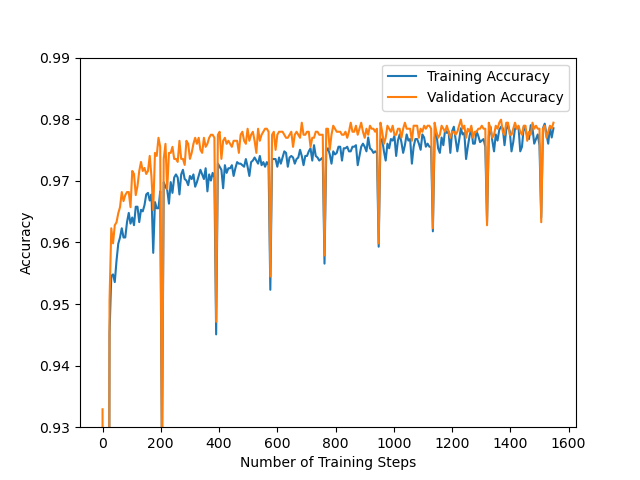
\includegraphics[width = \textwidth]{Assignment_1/Assignments/plots/task2abc/task2c_binary_train_accuracy.png}
    \caption{Accuracy for training and validation set for a given training step.}
    \label{fig:2caccuracy}
\end{figure}

\subsection{Task 2d: Early stopping}

To avoid overfitting the model to the training set, \textit{Early Stopping} has been implemented. By regularly checking if the loss for the validation set actually decreases, the training can be stopped early if the  validation loss has not decreased after a given set of checks. In this implementation, the training will stop if the loss does not decrease after passing 20\% of training data 10 times.

When training the model, it stopped after 33 epochs of a total 50 epochs due to the implementation of early stopping. Thus increasing the number of epochs from 50 to 500 has no practical effect.

The performance metrics for running the model in task2 with early stopping is shown in \autoref{table:metrics2}.
\begin{table}[H]
\centering
\begin{tabular}{|l|l|}
\hline

Final Train Cross Entropy Loss & 0.071           \\ \hline
Final Validation Cross Entropy Loss & 0.066           \\ \hline
Train accuracy           & 0.976         \\ \hline
Validation accuracy           & 0.979          \\ \hline
\end{tabular}
\caption{Performance metrics for the model after stopping at 33 epochs.}
\label{table:metrics2}
\end{table}


\subsection{Task 2e: Dataset shuffling}
The network convergence can be improved by shuffling the dataset between each epoch. This way, the network does not encounter the  exact same batch of examples each epoch. The effect of not shuffling the data in a neural network would be that the network memorises the training data, instead of creating a model that describes the data. This will result in overfitting and poor results on validation and test sets. By shuffling the data, different unique batches will be trained on the model, which will improve the gradient descent by having a more varied dataset. 

To clearly document the effect of shuffling the dataset, the validation accuracies with and without shuffle are shown in \autoref{fig:2eshuffle}. Additionally the training loss means and variances with and without shuffle are shown in \autoref{fig:2eshuffleloss}.

The shuffled training set yields less spikes in the accuracy and loss plots due to the fact that it has random orders on the training set. The spikes are due to batches that are disproportionately hard to classify. These batches, or maybe this one batch, has a set of images that are hard to classify and thus gives poor performance. By shuffling the data, we are not so unlucky to get this bad batch and therefore no huge spikes. 

\begin{figure}[H]
    \centering
    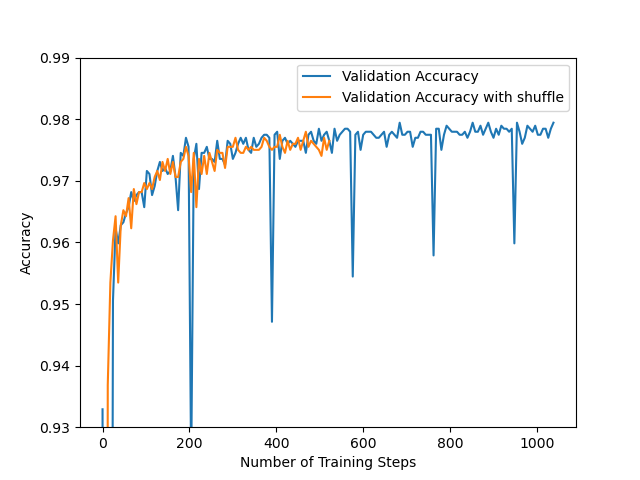
\includegraphics[width = \textwidth]{Assignment_1/Assignments/plots/task2de/task2e_train_accuracy_shuffle_difference.png}
    \caption{Accuracy of training with and without shuffled datasets.}
    
    \label{fig:2eshuffle}
\end{figure}
\begin{figure}[H]
    \centering
    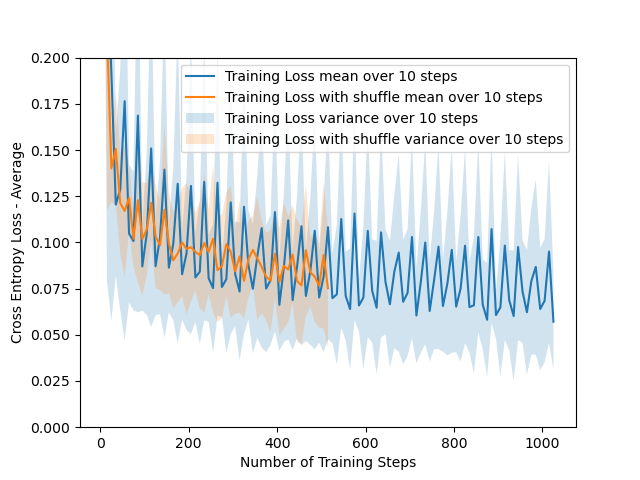
\includegraphics[width = \textwidth]{
Assignment_1/Assignments/plots/task2de/task2e_train_loss_with_shuffle.png}
    \caption{Training loss means and variances with and without shuffled datasets. }
    \label{fig:2eshuffleloss}
\end{figure}

\section{Softmax Regression through Gradient Descent}
\subsection{Task 3b: Training loss}

Softmax regression with mini-batch gradient descent for a single layer neural network has been implemented. During training, the training loss for each gradient step has been tracked. Additionally the validation loss over the whole validation set has been tracked for every time the network has progressed through 20\% of the training set. The loss results are shown in \autoref{fig:3bloss}. Here we clearly see a nice decrease in loss for the validation set with each iteration. For the training set however, even the mean over ten steps has quite high variance in loss. 

\begin{figure}[H]
    \centering
    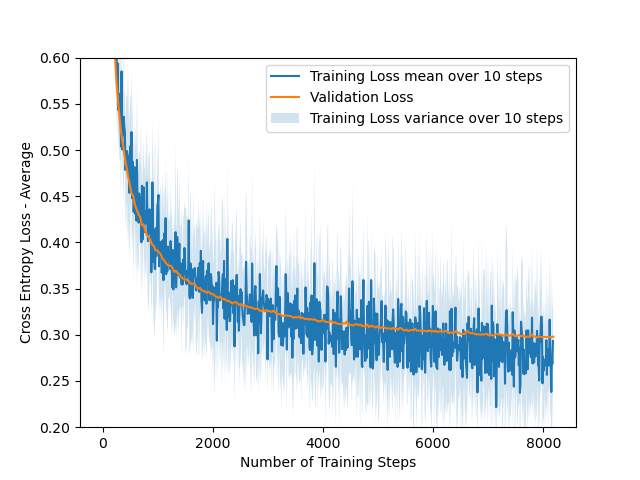
\includegraphics[width = \textwidth]{Assignment_1/Assignments/plots/task3/task3b_softmax_train_loss.png}
    \caption{Training loss and validation loss for Softmax regression with mini-batch gradient descent for a single layer neural network.}
    \label{fig:3bloss}
\end{figure}

\subsection{Task 3c: Accuracy}
A function computing the accuracy for both the training set and validation set has been implemented. The resulting accuracy plots for training and validation are shown in \autoref{fig:3caccuracy}. The plots show that after around 4000 training steps, the training accuracy improves significantly compared to the validation accuracy. This is further discussed in the next task.
\begin{figure}[H]
    \centering
    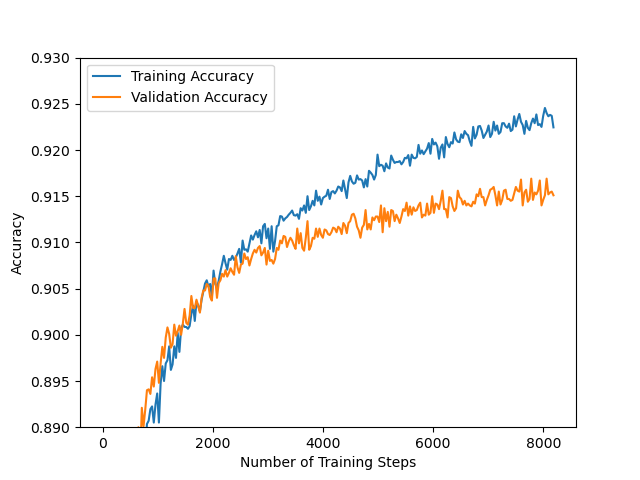
\includegraphics{Assignment_1/Assignments/plots/task3/task3b_softmax_train_accuracy.png}
    \caption{Prediction accuracy for the training set  and the validation set.}
    \label{fig:3caccuracy}
\end{figure}

\subsection{Task 3d: Overfitting}

From the accuracy plots shown in \autoref{fig:3caccuracy}, it is clear that the training accuracy is significantly better then the validation accuracy, after around 4000 training steps. This could be a sign of overfitting. If the training would continue for a longer period, the model could possibly begin to show worse performance on the validation set when increasing the training, and this would be considered overfitting. However, the accuracy for the validation and training set could both converg to a single common value or two different values. This is hard to tell from the plot.

\section{Regularization}

\subsection{Task 4a: Softmax gradient with $L_2$ regularization}

We wish to derive the new update term for our Softmax Regression after having introduced $L_2$ regression, given by

\begin{equation}
    J(w) = C(w) + \lambda R(w) \enskip , \enskip \lambda \in \mathbb{R}
\end{equation} 
where $C(w)$ is defined as

\begin{equation}
    C(w) = \frac{1}{N}\sum_{n=1}^N C^n(w)
\end{equation}
with $C^n(w)$ being the  multiple class cross entropy loss function defined in \eqref{eq:cn_def}. $R(w)$ is defined as the square of the $L_2$ norm of the weight matrix, $w$

\begin{equation}
    R(w) = \|w\|^2 = \sum_{i,j} w_{ij}^2
\end{equation}
The new update term will is given by $\frac{\partial J}{\partial w}$ In other words, we wish to compute

\begin{equation}
    \frac{\partial J}{\partial w} = \frac{\partial C(w)}{\partial w} + \lambda \frac{\partial R(w)}{\partial w}
    \label{eq:partial_j}
\end{equation}


Differentiating $C(w)$ gives:


\begin{align}
    \frac{\partial C(w)}{\partial w} &= \frac{\partial}{\partial w} \frac{1}{N} 
    \sum_{n=1}^N C^n(w) \\
    &= \frac{1}{N} \sum_{n=1}^N \frac{\partial}{\partial w} C^n(w) \\
\end{align}

Using the result from task 1b, we obtain

\begin{align}
    \frac{\partial C(w)}{\partial w} &= \frac{1}{N} \sum_{n=1}^N 
    \begin{bmatrix}
    \frac{\partial}{\partial w_{1,1}} C^n(w) & \frac{\partial}{\partial w_{1,2}} C^n(w) & \dots & \frac{\partial}{\partial w_{1,I}} C^n(w) \\
    \frac{\partial}{\partial w_{2,1}} C^n(w) & \frac{\partial}{\partial w_{2,2}} C^n(w)& \dots & \frac{\partial}{\partial w_{2,I}} C^n(w) \\
    \vdots & \vdots & \ddots & \vdots \\
    \frac{\partial}{\partial w_{K,1}} C^n(w) & \frac{\partial}{\partial w_{K,2}} \sum_{i,j}C^n(w)& \dots & \frac{\partial}{\partial w_{K,I}}C^n(w) \\
\end{bmatrix} \\
    &= \frac{1}{N} \sum_{n=1}^N  \begin{bmatrix}
    -x_1^n(y_1^n - \hat{y_1^n}) & -x_2^n(y_1^n - \hat{y_1^n}) & \dots & -x_I^n(y_1^n - \hat{y_1^n}) \\
    -x_1^n(y_2^n - \hat{y_2^n}) & -x_2^n(y_2^n - \hat{y_2^n}) & \dots & -x_I^n(y_2^n - \hat{y_2^n})  \\
    \vdots & \vdots & \ddots & \vdots \\
    -x_1^n(y_K^n - \hat{y_K^n}) & -x_2^n(y_K^n - \hat{y_K^n}) & \dots & -x_I^n(y_K^n - \hat{y_K^n}) \\
\end{bmatrix} \\
    &= \frac{1}{N} \sum_{n=1}^N \frac{\partial}{\partial w}C^n(w) \label{eq:dcw}
\end{align}

Differentiating $R(w)$ gives

\begin{align}
    \frac{\partial R(w)}{\partial w} &= \frac{\partial \|w\|^2}{\partial w} \\
    &= \frac{\partial}{\partial w} \sum_{i,j} w_{i,j}^2 \\
    &= \begin{bmatrix}
    \frac{\partial}{\partial w_{1,1}} \sum_{i,j} w_{i,j}^2 & \frac{\partial}{\partial w_{1,2}} \sum_{i,j} w_{i,j}^2 & \dots & \frac{\partial}{\partial w_{1,I}} \sum_{i,j} w_{i,j}^2 \\
    \frac{\partial}{\partial w_{2,1}} \sum_{i,j} w_{i,j}^2 & \frac{\partial}{\partial w_{2,2}} \sum_{i,j} w_{i,j}^2& \dots & \frac{\partial}{\partial w_{2,I}} \sum_{i,j}w_{i,j}^2 \\
    \vdots & \vdots & \ddots & \vdots \\
    \frac{\partial}{\partial w_{K,1}} \sum_{i,j} w_{i,j}^2 & \frac{\partial}{\partial w_{K,2}} \sum_{i,j} w_{i,j}^2& \dots & \frac{\partial}{\partial w_{K,I}} \sum_{i,j}w_{i,j}^2  \\
\end{bmatrix} \label{eq:matrix}
\end{align}

Considering the matrix in \eqref{eq:matrix}, similarly to in task 1a and 1b, the derivative for a given matrix entry, $\frac{\partial}{\partial w_{i',j'}} \sum_{i,j}w_{i,j}^2$ is only non-zero when $i' = i$ and $j'=j$. In that case the resulting matrix entry becomes $2w_{i',j'}$. Thus we can conclude that the derivative of $R(w)$ is


\begin{align}
    \frac{\partial R}{\partial w} &= 
    \begin{bmatrix}
    2w_{1,1} & 2w_{1,2}  & \dots & 2w_{1,I} \\
    2w_{2,1} & 2w_{2,2}  & \dots & 2w_{2,I} \\
    \vdots & \vdots & \ddots & \vdots \\
    2w_{K,1} & 2w_{K,2}  & \dots & 2w_{K,I} \\
\end{bmatrix} \\
    &= 2w \label{eq:drw}
\end{align}

where $w$ is the weight matrix.

Finally combining \eqref{eq:dcw} and \eqref{eq:drw} we obtain the new update term for the Softmax regression with $L_2$ regularization

\begin{equation}
    \frac{\partial J}{\partial w} = \frac{1}{N} \sum_{n=1}^N \frac{\partial}{\partial w}C^n(w) + 2\lambda w
\end{equation}

\subsection{Task 4b: Weights for different strengths of $L_2$ regularization}


In \autoref{fig:weight_clean} and \autoref{fig:weight_noisy} we have plotted the weights of a trained model with regularization. The parameter $\lambda$ used for the models is $0$ and $1$ respectively. Note that with $\lambda = 0$, the regularization is non existent. From the figures we clearly see that without regularization, $\lambda = 0$, the weights are more noisy. The weights with regularization, $\lambda = 1$ clearly resembles numbers. The point of regularization is to introduce some form of generalisation to the model, for instance noise, the goal of this is to make the model more general and not overfit. However in this example we see that the weights without regularization have the most noise, and thus look to be the most general. The regularization punishes the model for having weights with large magnitude. This is because having weights with smaller magnitude results in a simpler model, the model is then also considered to be more general. In our case we have a very simple network with only one layer. Therefore the model is simply to simple and the weights to sparse, when $\lambda$ is large. However, if the model was more complex, more layers, things might have been different, and a larger $\lambda$ would be beneficial. 


 \begin{figure}[H]
     \centering
     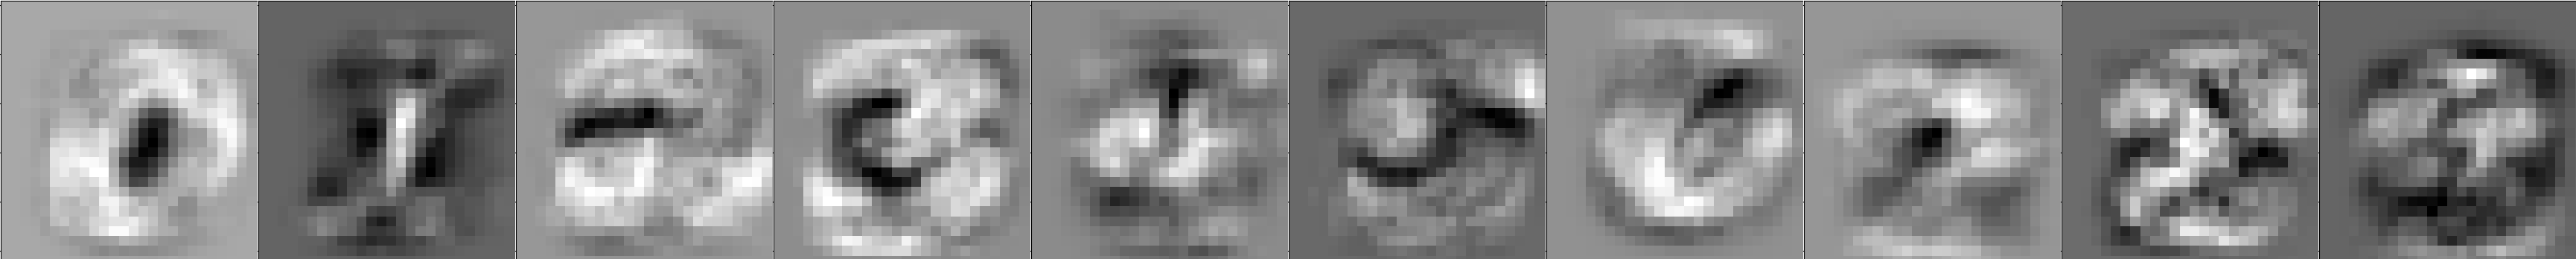
\includegraphics[width=\textwidth]{Assignment_1/Assignments/plots/task4/task4b_softmax_weight_0l_.png}
     \caption{Combined 28x28 plot of all the weights without biases with $\lambda = 0$}
     \label{fig:weight_noisy}
 \end{figure}
 
  \begin{figure}[H]
     \centering
     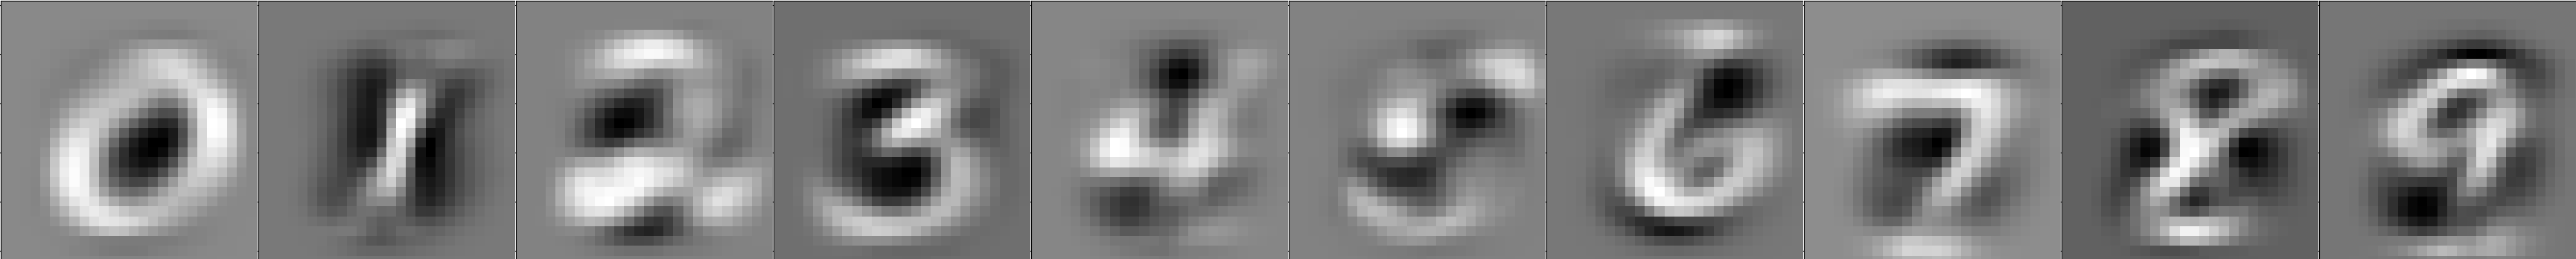
\includegraphics[width=\textwidth]{Assignment_1/Assignments/plots/task4/task4b_softmax_weight_1l_.png}
     \caption{Combined 28x28 plot of all the weights without biases with $\lambda = 1$}
     \label{fig:weight_clean}
 \end{figure}
 
\subsection{Task 4c: Validation accuracy for different strengths of $L_2$ regularization }
The accuracy for the model with the given values of lambda $\lambda= \{0, 0.001, 0.01, 0.1, 1\}$ is shown in \autoref{fig:lambda-acc}.

\begin{figure}[H]
    \centering
    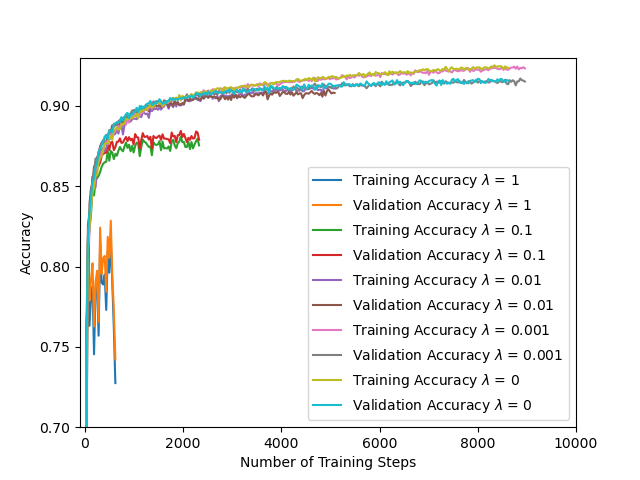
\includegraphics[width=\textwidth]{Assignment_1/Assignments/plots/task4/task4c_l2_reg_accuracy.png}
    \caption{Accuracies for a trained model with regularisation for different values of $\lambda$}
    \label{fig:lambda-acc}
\end{figure}

\subsection{Task 4d: Degrading validation accuracy for different strengths of $L_2$ regularization}
It is clear that the accuracy for both sets, training and validation, degrades when increasing $\lambda$. This is expected when taking in consideration what was stated in task 4b. The regularization has the wanted effect of making the model simpler, however the model becomes too simple with weights that are too small for the classification task. Thus the performance becomes worse when increasing the regularization.


\subsection{Task 4e: $L_2$ Norm}
In \autoref{fig:norm} the norm of the weights is plotted against $\lambda$, here we clearly see the effect first mentioned in 4b. The regularization simplifies the model and thus also reduces the norm of $w$. The regularization does exactly what it is intended to do, but in our particular case, does not yield good results. 

\begin{figure}[H]
    \centering
    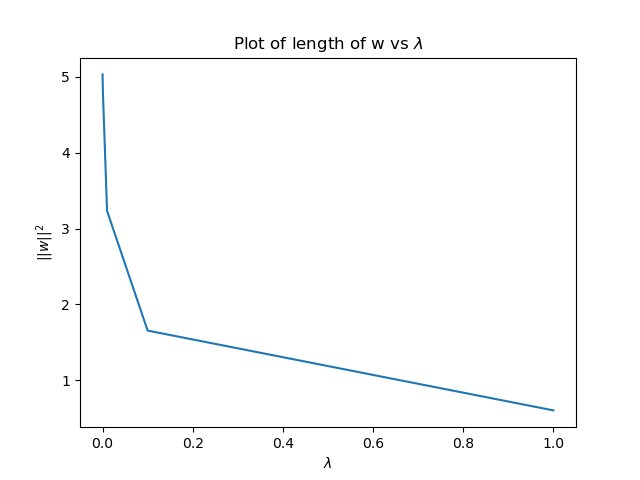
\includegraphics{Assignment_1/Assignments/plots/task4/task4d_l2_reg_norms.png}
    \caption{Plot showing the $L_2$ norm of the weights against the lambda values $\lambda= \{0, 0.001, 0.01, 0.1, 1\}$ }
    \label{fig:norm}
\end{figure}


\end{document}